\documentclass[twoside]{book}

% Packages required by doxygen
\usepackage{fixltx2e}
\usepackage{calc}
\usepackage{doxygen}
\usepackage[export]{adjustbox} % also loads graphicx
\usepackage{graphicx}
\usepackage[utf8]{inputenc}
\usepackage{makeidx}
\usepackage{multicol}
\usepackage{multirow}
\PassOptionsToPackage{warn}{textcomp}
\usepackage{textcomp}
\usepackage[nointegrals]{wasysym}
\usepackage[table]{xcolor}

% Font selection
\usepackage[T1]{fontenc}
\usepackage[scaled=.90]{helvet}
\usepackage{courier}
\usepackage{amssymb}
\usepackage{sectsty}
\renewcommand{\familydefault}{\sfdefault}
\allsectionsfont{%
  \fontseries{bc}\selectfont%
  \color{darkgray}%
}
\renewcommand{\DoxyLabelFont}{%
  \fontseries{bc}\selectfont%
  \color{darkgray}%
}
\newcommand{\+}{\discretionary{\mbox{\scriptsize$\hookleftarrow$}}{}{}}

% Page & text layout
\usepackage{geometry}
\geometry{%
  a4paper,%
  top=2.5cm,%
  bottom=2.5cm,%
  left=2.5cm,%
  right=2.5cm%
}
\tolerance=750
\hfuzz=15pt
\hbadness=750
\setlength{\emergencystretch}{15pt}
\setlength{\parindent}{0cm}
\setlength{\parskip}{3ex plus 2ex minus 2ex}
\makeatletter
\renewcommand{\paragraph}{%
  \@startsection{paragraph}{4}{0ex}{-1.0ex}{1.0ex}{%
    \normalfont\normalsize\bfseries\SS@parafont%
  }%
}
\renewcommand{\subparagraph}{%
  \@startsection{subparagraph}{5}{0ex}{-1.0ex}{1.0ex}{%
    \normalfont\normalsize\bfseries\SS@subparafont%
  }%
}
\makeatother

% Headers & footers
\usepackage{fancyhdr}
\pagestyle{fancyplain}
\fancyhead[LE]{\fancyplain{}{\bfseries\thepage}}
\fancyhead[CE]{\fancyplain{}{}}
\fancyhead[RE]{\fancyplain{}{\bfseries\leftmark}}
\fancyhead[LO]{\fancyplain{}{\bfseries\rightmark}}
\fancyhead[CO]{\fancyplain{}{}}
\fancyhead[RO]{\fancyplain{}{\bfseries\thepage}}
\fancyfoot[LE]{\fancyplain{}{}}
\fancyfoot[CE]{\fancyplain{}{}}
\fancyfoot[RE]{\fancyplain{}{\bfseries\scriptsize Generated by Doxygen }}
\fancyfoot[LO]{\fancyplain{}{\bfseries\scriptsize Generated by Doxygen }}
\fancyfoot[CO]{\fancyplain{}{}}
\fancyfoot[RO]{\fancyplain{}{}}
\renewcommand{\footrulewidth}{0.4pt}
\renewcommand{\chaptermark}[1]{%
  \markboth{#1}{}%
}
\renewcommand{\sectionmark}[1]{%
  \markright{\thesection\ #1}%
}

% Indices & bibliography
\usepackage{natbib}
\usepackage[titles]{tocloft}
\setcounter{tocdepth}{3}
\setcounter{secnumdepth}{5}
\makeindex

% Hyperlinks (required, but should be loaded last)
\usepackage{ifpdf}
\ifpdf
  \usepackage[pdftex,pagebackref=true]{hyperref}
\else
  \usepackage[ps2pdf,pagebackref=true]{hyperref}
\fi
\hypersetup{%
  colorlinks=true,%
  linkcolor=blue,%
  citecolor=blue,%
  unicode%
}

% Custom commands
\newcommand{\clearemptydoublepage}{%
  \newpage{\pagestyle{empty}\cleardoublepage}%
}

\usepackage{caption}
\captionsetup{labelsep=space,justification=centering,font={bf},singlelinecheck=off,skip=4pt,position=top}

%===== C O N T E N T S =====

\begin{document}

% Titlepage & ToC
\hypersetup{pageanchor=false,
             bookmarksnumbered=true,
             pdfencoding=unicode
            }
\pagenumbering{alph}
\begin{titlepage}
\vspace*{7cm}
\begin{center}%
{\Large My Project }\\
\vspace*{1cm}
{\large Generated by Doxygen 1.8.14}\\
\end{center}
\end{titlepage}
\clearemptydoublepage
\pagenumbering{roman}
\tableofcontents
\clearemptydoublepage
\pagenumbering{arabic}
\hypersetup{pageanchor=true}

%--- Begin generated contents ---
\chapter{Hierarchical Index}
\section{Class Hierarchy}
This inheritance list is sorted roughly, but not completely, alphabetically\+:\begin{DoxyCompactList}
\item Mono\+Behaviour\begin{DoxyCompactList}
\item \contentsline{section}{antiportal}{\pageref{classantiportal}}{}
\item \contentsline{section}{Box\+Movement}{\pageref{class_box_movement}}{}
\item \contentsline{section}{Button}{\pageref{class_button}}{}
\item \contentsline{section}{chip\+AI}{\pageref{classchip_a_i}}{}
\item \contentsline{section}{Collision\+Detection}{\pageref{class_collision_detection}}{}
\item \contentsline{section}{Collision\+Detection}{\pageref{class_collision_detection}}{}
\item \contentsline{section}{Collision\+Detection}{\pageref{class_collision_detection}}{}
\item \contentsline{section}{Collision\+Detection}{\pageref{class_collision_detection}}{}
\item \contentsline{section}{Game\+Manager}{\pageref{class_game_manager}}{}
\item \contentsline{section}{Game\+Manager}{\pageref{class_game_manager}}{}
\item \contentsline{section}{Game\+Manager}{\pageref{class_game_manager}}{}
\item \contentsline{section}{Game\+Manager}{\pageref{class_game_manager}}{}
\item \contentsline{section}{Gun\+Rotation}{\pageref{class_gun_rotation}}{}
\item \contentsline{section}{Gun\+Rotation}{\pageref{class_gun_rotation}}{}
\item \contentsline{section}{Gun\+Rotation}{\pageref{class_gun_rotation}}{}
\item \contentsline{section}{Gun\+Rotation}{\pageref{class_gun_rotation}}{}
\item \contentsline{section}{hazard}{\pageref{classhazard}}{}
\item \contentsline{section}{Level\+Selector}{\pageref{class_level_selector}}{}
\item \contentsline{section}{Main\+Menu}{\pageref{class_main_menu}}{}
\item \contentsline{section}{open\+\_\+\+Door}{\pageref{classopen___door}}{}
\item \contentsline{section}{open\+\_\+\+Door}{\pageref{classopen___door}}{}
\item \contentsline{section}{open\+\_\+\+Door}{\pageref{classopen___door}}{}
\item \contentsline{section}{open\+\_\+\+Door}{\pageref{classopen___door}}{}
\item \contentsline{section}{Pause}{\pageref{class_pause}}{}
\item \contentsline{section}{Player\+Movement}{\pageref{class_player_movement}}{}
\item \contentsline{section}{Player\+Movement}{\pageref{class_player_movement}}{}
\item \contentsline{section}{Player\+Movement}{\pageref{class_player_movement}}{}
\item \contentsline{section}{Player\+Movement}{\pageref{class_player_movement}}{}
\item \contentsline{section}{Portal\+Movement}{\pageref{class_portal_movement}}{}
\item \contentsline{section}{Portal\+Movement}{\pageref{class_portal_movement}}{}
\item \contentsline{section}{Portal\+Movement}{\pageref{class_portal_movement}}{}
\item \contentsline{section}{Portal\+Movement}{\pageref{class_portal_movement}}{}
\item \contentsline{section}{Shoot\+Portal}{\pageref{class_shoot_portal}}{}
\item \contentsline{section}{Shoot\+Portal}{\pageref{class_shoot_portal}}{}
\item \contentsline{section}{Shoot\+Portal}{\pageref{class_shoot_portal}}{}
\item \contentsline{section}{Shoot\+Portal}{\pageref{class_shoot_portal}}{}
\item \contentsline{section}{Teleport\+Box}{\pageref{class_teleport_box}}{}
\item \contentsline{section}{teleporter\+Location}{\pageref{classteleporter_location}}{}
\item \contentsline{section}{Teleport\+Player}{\pageref{class_teleport_player}}{}
\item \contentsline{section}{Teleport\+Player}{\pageref{class_teleport_player}}{}
\item \contentsline{section}{Teleport\+Player}{\pageref{class_teleport_player}}{}
\item \contentsline{section}{Teleport\+Player}{\pageref{class_teleport_player}}{}
\item \contentsline{section}{Win\+Game}{\pageref{class_win_game}}{}
\item \contentsline{section}{Win\+Game}{\pageref{class_win_game}}{}
\item \contentsline{section}{Win\+Game}{\pageref{class_win_game}}{}
\item \contentsline{section}{Win\+Game}{\pageref{class_win_game}}{}
\end{DoxyCompactList}
\end{DoxyCompactList}

\chapter{Class Index}
\section{Class List}
Here are the classes, structs, unions and interfaces with brief descriptions\+:\begin{DoxyCompactList}
\item\contentsline{section}{\mbox{\hyperlink{classantiportal}{antiportal}} }{\pageref{classantiportal}}{}
\item\contentsline{section}{\mbox{\hyperlink{class_box_movement}{Box\+Movement}} }{\pageref{class_box_movement}}{}
\item\contentsline{section}{\mbox{\hyperlink{class_button}{Button}} }{\pageref{class_button}}{}
\item\contentsline{section}{\mbox{\hyperlink{classchip_a_i}{chip\+AI}} }{\pageref{classchip_a_i}}{}
\item\contentsline{section}{\mbox{\hyperlink{class_collision_detection}{Collision\+Detection}} }{\pageref{class_collision_detection}}{}
\item\contentsline{section}{\mbox{\hyperlink{class_game_manager}{Game\+Manager}} }{\pageref{class_game_manager}}{}
\item\contentsline{section}{\mbox{\hyperlink{class_gun_rotation}{Gun\+Rotation}} }{\pageref{class_gun_rotation}}{}
\item\contentsline{section}{\mbox{\hyperlink{classhazard}{hazard}} }{\pageref{classhazard}}{}
\item\contentsline{section}{\mbox{\hyperlink{class_level_selector}{Level\+Selector}} }{\pageref{class_level_selector}}{}
\item\contentsline{section}{\mbox{\hyperlink{class_main_menu}{Main\+Menu}} }{\pageref{class_main_menu}}{}
\item\contentsline{section}{\mbox{\hyperlink{classopen___door}{open\+\_\+\+Door}} }{\pageref{classopen___door}}{}
\item\contentsline{section}{\mbox{\hyperlink{class_pause}{Pause}} }{\pageref{class_pause}}{}
\item\contentsline{section}{\mbox{\hyperlink{class_player_movement}{Player\+Movement}} }{\pageref{class_player_movement}}{}
\item\contentsline{section}{\mbox{\hyperlink{class_portal_movement}{Portal\+Movement}} }{\pageref{class_portal_movement}}{}
\item\contentsline{section}{\mbox{\hyperlink{class_shoot_portal}{Shoot\+Portal}} }{\pageref{class_shoot_portal}}{}
\item\contentsline{section}{\mbox{\hyperlink{class_teleport_box}{Teleport\+Box}} }{\pageref{class_teleport_box}}{}
\item\contentsline{section}{\mbox{\hyperlink{classteleporter_location}{teleporter\+Location}} }{\pageref{classteleporter_location}}{}
\item\contentsline{section}{\mbox{\hyperlink{class_teleport_player}{Teleport\+Player}} }{\pageref{class_teleport_player}}{}
\item\contentsline{section}{\mbox{\hyperlink{class_win_game}{Win\+Game}} }{\pageref{class_win_game}}{}
\end{DoxyCompactList}

\chapter{Class Documentation}
\hypertarget{class_collision_detection}{}\section{Collision\+Detection Class Reference}
\label{class_collision_detection}\index{Collision\+Detection@{Collision\+Detection}}
Inheritance diagram for Collision\+Detection\+:\begin{figure}[H]
\begin{center}
\leavevmode
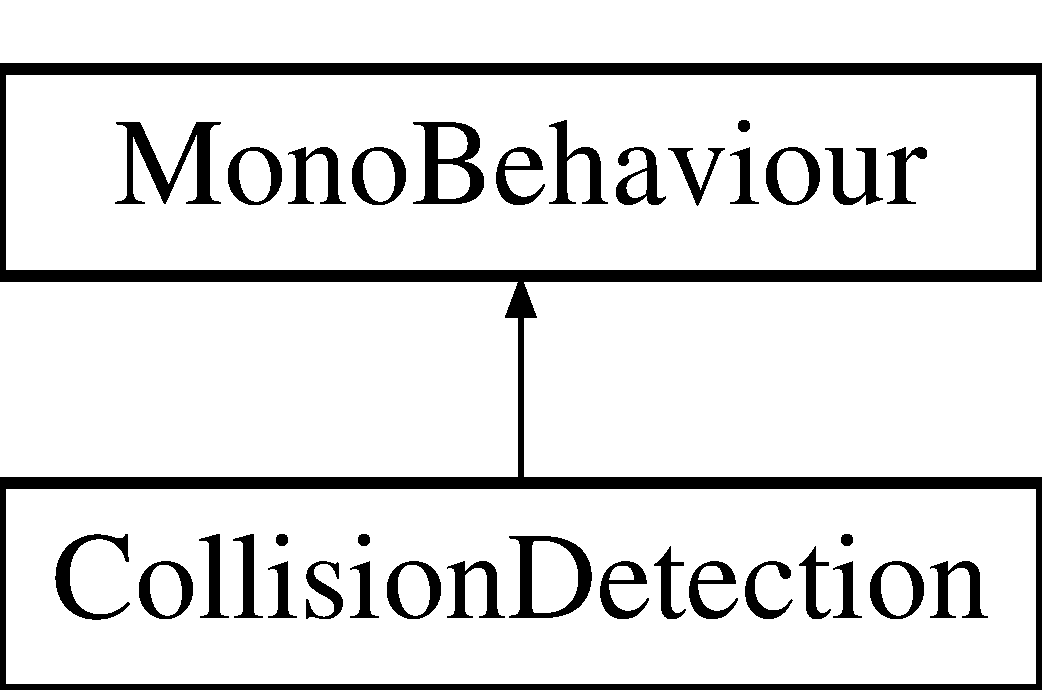
\includegraphics[height=2.000000cm]{class_collision_detection}
\end{center}
\end{figure}
\subsection*{Public Member Functions}
\begin{DoxyCompactItemize}
\item 
void \mbox{\hyperlink{class_collision_detection_ae5c7d4d990b3c888dc8866821a3d0366}{On\+Collision\+Enter2D}} (Collision2D collision)
\item 
void \mbox{\hyperlink{class_collision_detection_ae5c7d4d990b3c888dc8866821a3d0366}{On\+Collision\+Enter2D}} (Collision2D collision)
\end{DoxyCompactItemize}
\subsection*{Public Attributes}
\begin{DoxyCompactItemize}
\item 
\mbox{\Hypertarget{class_collision_detection_a5998d298c2f3c52ca58af7e2604a8559}\label{class_collision_detection_a5998d298c2f3c52ca58af7e2604a8559}} 
Game\+Object {\bfseries blue\+Portal}
\item 
\mbox{\Hypertarget{class_collision_detection_acb663162929e709c69b80cf62f864d6a}\label{class_collision_detection_acb663162929e709c69b80cf62f864d6a}} 
Game\+Object {\bfseries red\+Portal}
\item 
\mbox{\Hypertarget{class_collision_detection_a4bd58b38fd8034d725f0262c78addfeb}\label{class_collision_detection_a4bd58b38fd8034d725f0262c78addfeb}} 
Game\+Object {\bfseries Portal}
\item 
\mbox{\Hypertarget{class_collision_detection_a4281fd2d4607ab7b94d947928dc388a9}\label{class_collision_detection_a4281fd2d4607ab7b94d947928dc388a9}} 
Game\+Object {\bfseries New\+Portal}
\end{DoxyCompactItemize}


\subsection{Detailed Description}
Handles collision of portal bullet with terrain. 

\subsection{Member Function Documentation}
\mbox{\Hypertarget{class_collision_detection_ae5c7d4d990b3c888dc8866821a3d0366}\label{class_collision_detection_ae5c7d4d990b3c888dc8866821a3d0366}} 
\index{Collision\+Detection@{Collision\+Detection}!On\+Collision\+Enter2D@{On\+Collision\+Enter2D}}
\index{On\+Collision\+Enter2D@{On\+Collision\+Enter2D}!Collision\+Detection@{Collision\+Detection}}
\subsubsection{\texorpdfstring{On\+Collision\+Enter2\+D()}{OnCollisionEnter2D()}\hspace{0.1cm}{\footnotesize\ttfamily [1/2]}}
{\footnotesize\ttfamily void Collision\+Detection.\+On\+Collision\+Enter2D (\begin{DoxyParamCaption}\item[{Collision2D}]{collision }\end{DoxyParamCaption})\hspace{0.3cm}{\ttfamily [inline]}}

This method runs when the portal bullet hits a surface generating a collision. \begin{DoxyPrecond}{Precondition}
portal bullet is shot 
\end{DoxyPrecond}
\begin{DoxyPostcond}{Postcondition}
after collision with appropriate surface portal gets created and previous portal gets destroyed 
\end{DoxyPostcond}
\mbox{\Hypertarget{class_collision_detection_ae5c7d4d990b3c888dc8866821a3d0366}\label{class_collision_detection_ae5c7d4d990b3c888dc8866821a3d0366}} 
\index{Collision\+Detection@{Collision\+Detection}!On\+Collision\+Enter2D@{On\+Collision\+Enter2D}}
\index{On\+Collision\+Enter2D@{On\+Collision\+Enter2D}!Collision\+Detection@{Collision\+Detection}}
\subsubsection{\texorpdfstring{On\+Collision\+Enter2\+D()}{OnCollisionEnter2D()}\hspace{0.1cm}{\footnotesize\ttfamily [2/2]}}
{\footnotesize\ttfamily void Collision\+Detection.\+On\+Collision\+Enter2D (\begin{DoxyParamCaption}\item[{Collision2D}]{collision }\end{DoxyParamCaption})\hspace{0.3cm}{\ttfamily [inline]}}

This method runs when the portal bullet hits a surface generating a collision. \begin{DoxyPrecond}{Precondition}
portal bullet is shot 
\end{DoxyPrecond}
\begin{DoxyPostcond}{Postcondition}
after collision with appropriate surface portal gets created and previous portal gets destroyed 
\end{DoxyPostcond}

\begin{DoxyParams}{Parameters}
{\em collision} & collision object created by the physics engine \\
\hline
\end{DoxyParams}


The documentation for this class was generated from the following file\+:\begin{DoxyCompactItemize}
\item 
Assets/\+Scripts/Collision\+Detection.\+cs\end{DoxyCompactItemize}

\hypertarget{class_game_manager}{}\section{Game\+Manager Class Reference}
\label{class_game_manager}\index{Game\+Manager@{Game\+Manager}}
Inheritance diagram for Game\+Manager\+:\begin{figure}[H]
\begin{center}
\leavevmode
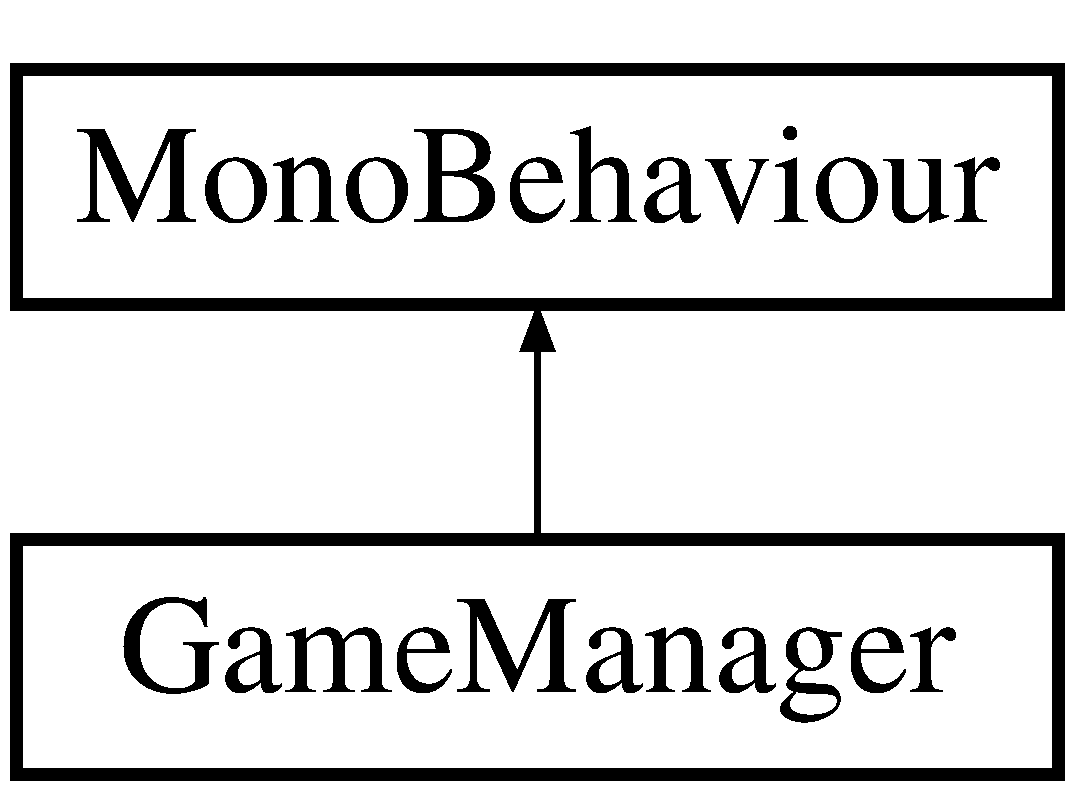
\includegraphics[height=2.000000cm]{class_game_manager}
\end{center}
\end{figure}
\subsection*{Public Member Functions}
\begin{DoxyCompactItemize}
\item 
void \mbox{\hyperlink{class_game_manager_a5ccfacd027ad08eeb4ff1f25a7f59c98}{Start}} ()
\item 
void \mbox{\hyperlink{class_game_manager_a76a27f36d082e328bd1c7748d8832816}{Win}} ()
\end{DoxyCompactItemize}
\subsection*{Public Attributes}
\begin{DoxyCompactItemize}
\item 
\mbox{\Hypertarget{class_game_manager_a9e2addf3b88748a4d46a5428e1e332f0}\label{class_game_manager_a9e2addf3b88748a4d46a5428e1e332f0}} 
Game\+Object {\bfseries you\+Win}
\end{DoxyCompactItemize}
\subsection*{Static Public Attributes}
\begin{DoxyCompactItemize}
\item 
\mbox{\Hypertarget{class_game_manager_a7666e8468dac197b9eb32dd32128524f}\label{class_game_manager_a7666e8468dac197b9eb32dd32128524f}} 
static \mbox{\hyperlink{class_game_manager}{Game\+Manager}} {\bfseries instance} = null
\end{DoxyCompactItemize}


\subsection{Detailed Description}
Handles game instance. 

\subsection{Member Function Documentation}
\mbox{\Hypertarget{class_game_manager_a5ccfacd027ad08eeb4ff1f25a7f59c98}\label{class_game_manager_a5ccfacd027ad08eeb4ff1f25a7f59c98}} 
\index{Game\+Manager@{Game\+Manager}!Start@{Start}}
\index{Start@{Start}!Game\+Manager@{Game\+Manager}}
\subsubsection{\texorpdfstring{Start()}{Start()}}
{\footnotesize\ttfamily void Game\+Manager.\+Start (\begin{DoxyParamCaption}{ }\end{DoxyParamCaption})\hspace{0.3cm}{\ttfamily [inline]}}

Runs at start. \begin{DoxyPrecond}{Precondition}
game starts 
\end{DoxyPrecond}
\begin{DoxyPostcond}{Postcondition}
Instance of the game is created 
\end{DoxyPostcond}
\mbox{\Hypertarget{class_game_manager_a76a27f36d082e328bd1c7748d8832816}\label{class_game_manager_a76a27f36d082e328bd1c7748d8832816}} 
\index{Game\+Manager@{Game\+Manager}!Win@{Win}}
\index{Win@{Win}!Game\+Manager@{Game\+Manager}}
\subsubsection{\texorpdfstring{Win()}{Win()}}
{\footnotesize\ttfamily void Game\+Manager.\+Win (\begin{DoxyParamCaption}{ }\end{DoxyParamCaption})\hspace{0.3cm}{\ttfamily [inline]}}

Sets win state to true. function is called by \mbox{\hyperlink{class_win_game}{Win\+Game()}} \begin{DoxyPrecond}{Precondition}
User reached door object 
\end{DoxyPrecond}
\begin{DoxyPostcond}{Postcondition}
Success message is displayed 
\end{DoxyPostcond}


The documentation for this class was generated from the following file\+:\begin{DoxyCompactItemize}
\item 
Assets/\+Scripts/Game\+Manager.\+cs\end{DoxyCompactItemize}

\hypertarget{class_gun_rotation}{}\section{Gun\+Rotation Class Reference}
\label{class_gun_rotation}\index{Gun\+Rotation@{Gun\+Rotation}}
Inheritance diagram for Gun\+Rotation\+:\begin{figure}[H]
\begin{center}
\leavevmode
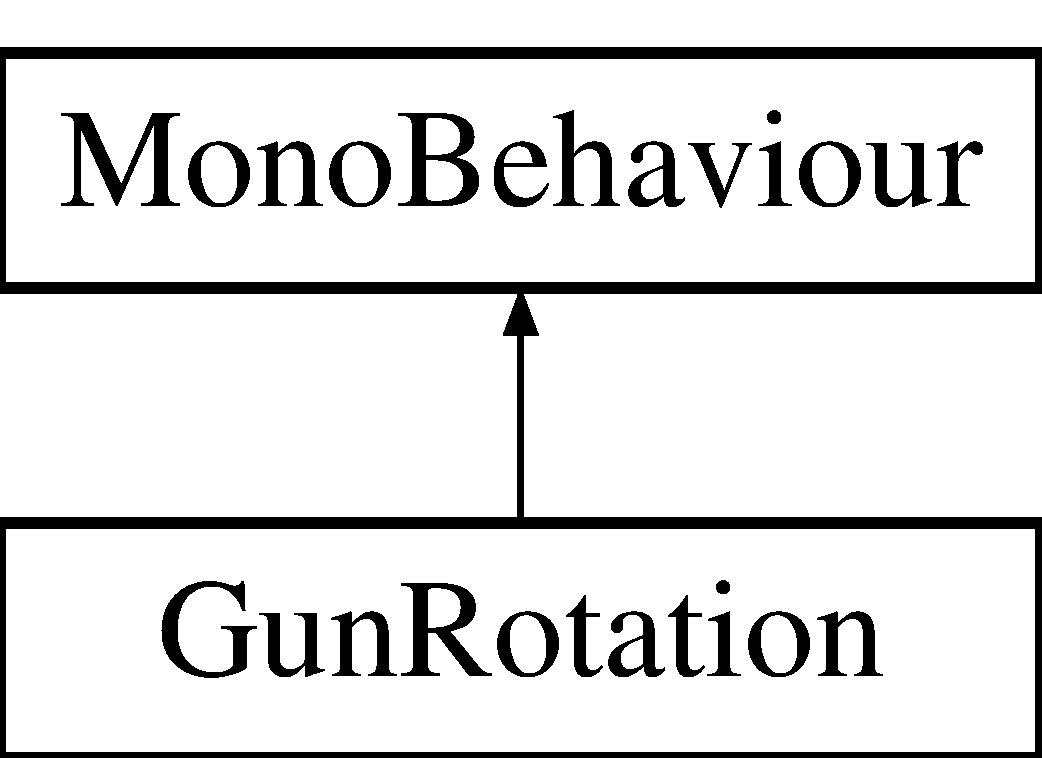
\includegraphics[height=2.000000cm]{class_gun_rotation}
\end{center}
\end{figure}


\subsection{Detailed Description}
Aims gun at mouse cursor. 

The documentation for this class was generated from the following file\+:\begin{DoxyCompactItemize}
\item 
Assets/\+Scripts/Gun\+Rotation.\+cs\end{DoxyCompactItemize}

\hypertarget{classopen___door}{}\section{open\+\_\+\+Door Class Reference}
\label{classopen___door}\index{open\+\_\+\+Door@{open\+\_\+\+Door}}
Inheritance diagram for open\+\_\+\+Door\+:\begin{figure}[H]
\begin{center}
\leavevmode
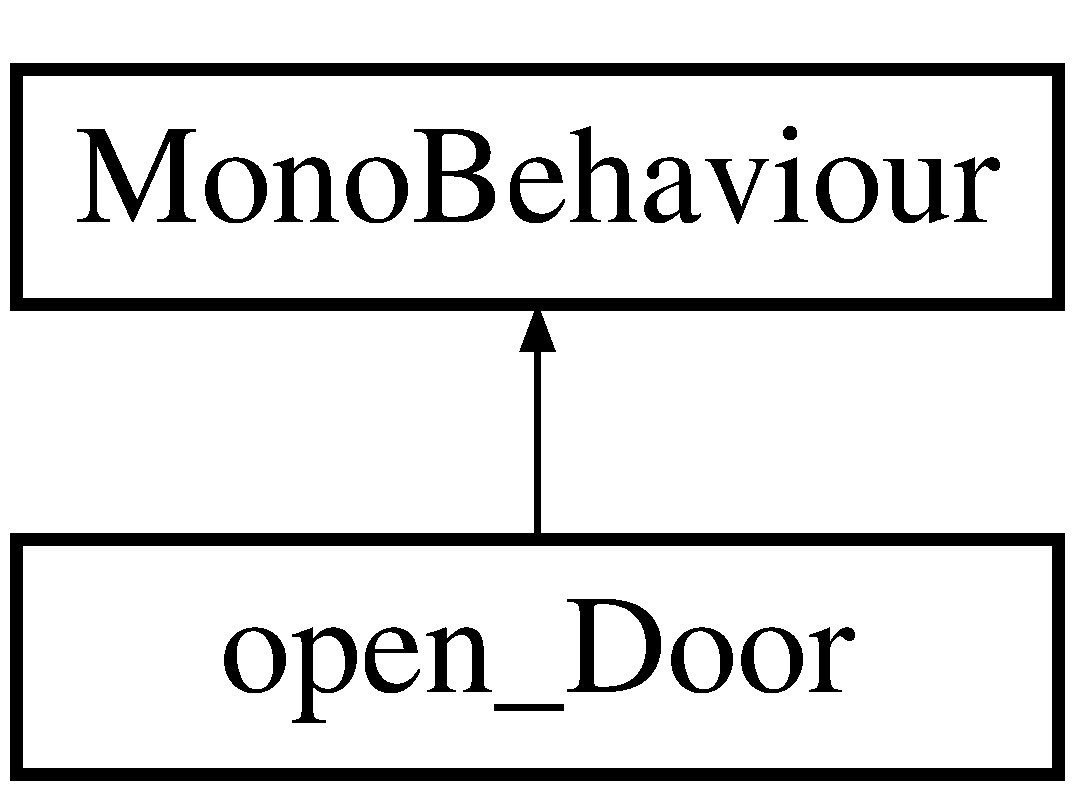
\includegraphics[height=2.000000cm]{classopen___door}
\end{center}
\end{figure}
\subsection*{Public Member Functions}
\begin{DoxyCompactItemize}
\item 
\mbox{\Hypertarget{classopen___door_a73d16144fb87c086186bd5c26b5919a5}\label{classopen___door_a73d16144fb87c086186bd5c26b5919a5}} 
void {\bfseries Start} ()
\item 
\mbox{\Hypertarget{classopen___door_a7689f551c5c3a63718e506e6e101c36f}\label{classopen___door_a7689f551c5c3a63718e506e6e101c36f}} 
void {\bfseries Update} ()
\item 
void \mbox{\hyperlink{classopen___door_af445b9df0f862ee2c2d667d6b1f92811}{player\+Hits\+Door}} (Collision2D collision)
\end{DoxyCompactItemize}
\subsection*{Public Attributes}
\begin{DoxyCompactItemize}
\item 
\mbox{\Hypertarget{classopen___door_afdfd02e742a29a8091cc062da7ebf335}\label{classopen___door_afdfd02e742a29a8091cc062da7ebf335}} 
bool {\bfseries door\+Is\+Open} = false
\item 
\mbox{\Hypertarget{classopen___door_a2d7b03a65ed29ef63bd7d17a19b57404}\label{classopen___door_a2d7b03a65ed29ef63bd7d17a19b57404}} 
Game\+Object {\bfseries Door}
\end{DoxyCompactItemize}


\subsection{Detailed Description}
Opens final door. 

\subsection{Member Function Documentation}
\mbox{\Hypertarget{classopen___door_af445b9df0f862ee2c2d667d6b1f92811}\label{classopen___door_af445b9df0f862ee2c2d667d6b1f92811}} 
\index{open\+\_\+\+Door@{open\+\_\+\+Door}!player\+Hits\+Door@{player\+Hits\+Door}}
\index{player\+Hits\+Door@{player\+Hits\+Door}!open\+\_\+\+Door@{open\+\_\+\+Door}}
\subsubsection{\texorpdfstring{player\+Hits\+Door()}{playerHitsDoor()}}
{\footnotesize\ttfamily void open\+\_\+\+Door.\+player\+Hits\+Door (\begin{DoxyParamCaption}\item[{Collision2D}]{collision }\end{DoxyParamCaption})\hspace{0.3cm}{\ttfamily [inline]}}

will start animation after player collides with exit door indicating level was completed. 

The documentation for this class was generated from the following file\+:\begin{DoxyCompactItemize}
\item 
Assets/\+Scripts/open\+\_\+\+Door.\+cs\end{DoxyCompactItemize}

\hypertarget{class_player_movement}{}\section{Player\+Movement Class Reference}
\label{class_player_movement}\index{Player\+Movement@{Player\+Movement}}
Inheritance diagram for Player\+Movement\+:\begin{figure}[H]
\begin{center}
\leavevmode
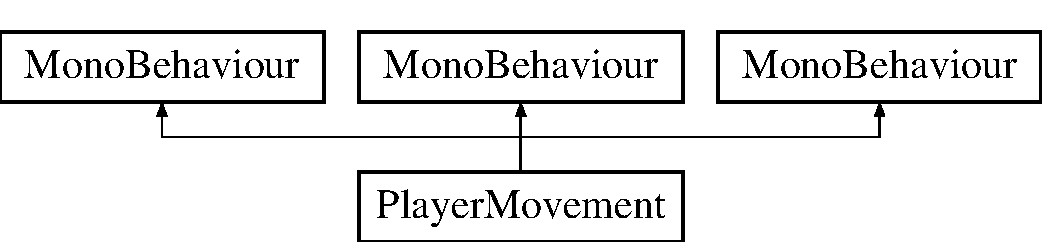
\includegraphics[height=2.000000cm]{class_player_movement}
\end{center}
\end{figure}
\subsection*{Public Member Functions}
\begin{DoxyCompactItemize}
\item 
void \mbox{\hyperlink{class_player_movement_abf3660ca2b1a352b4a9da98437c61aa3}{Start}} ()
\item 
void \mbox{\hyperlink{class_player_movement_aaf9b77d7177d538be9c1447d08191322}{Update}} ()
\item 
void \mbox{\hyperlink{class_player_movement_a0caaa871b9ef680c9f02bd0e22c77db1}{Fixed\+Update}} ()
\item 
void \mbox{\hyperlink{class_player_movement_aea65f5f7247feb09772da2543c8ec427}{Direction\+Switch}} ()
\end{DoxyCompactItemize}
\subsection*{Public Attributes}
\begin{DoxyCompactItemize}
\item 
\mbox{\Hypertarget{class_player_movement_aa83a2390fe399c816eac24ac74a02528}\label{class_player_movement_aa83a2390fe399c816eac24ac74a02528}} 
bool {\bfseries face\+Right} = true
\item 
\mbox{\Hypertarget{class_player_movement_aaf3e5c59c7392a57747a6a189c29febe}\label{class_player_movement_aaf3e5c59c7392a57747a6a189c29febe}} 
bool {\bfseries jump} = false
\item 
\mbox{\Hypertarget{class_player_movement_a411dc41a76270f4ff0ea15e0b996b8ed}\label{class_player_movement_a411dc41a76270f4ff0ea15e0b996b8ed}} 
float {\bfseries move\+Force} = 365f
\item 
\mbox{\Hypertarget{class_player_movement_a18b9bde59ef4f50acf685694f67ee3c7}\label{class_player_movement_a18b9bde59ef4f50acf685694f67ee3c7}} 
float {\bfseries max\+Speed} = 5f
\item 
\mbox{\Hypertarget{class_player_movement_a2918af247f8fd93a1dfe84b8d997c280}\label{class_player_movement_a2918af247f8fd93a1dfe84b8d997c280}} 
float {\bfseries jump\+Force} = 200f
\item 
\mbox{\Hypertarget{class_player_movement_a681e7b28ce40d859bbe21c231a676ce8}\label{class_player_movement_a681e7b28ce40d859bbe21c231a676ce8}} 
Transform {\bfseries ground\+Check}
\item 
\mbox{\Hypertarget{class_player_movement_a48a8923fa5137614141dd6886257af61}\label{class_player_movement_a48a8923fa5137614141dd6886257af61}} 
bool {\bfseries is\+Teleported} = false
\end{DoxyCompactItemize}


\subsection{Detailed Description}
Handles player movement. 

\subsection{Member Function Documentation}
\mbox{\Hypertarget{class_player_movement_aea65f5f7247feb09772da2543c8ec427}\label{class_player_movement_aea65f5f7247feb09772da2543c8ec427}} 
\index{Player\+Movement@{Player\+Movement}!Direction\+Switch@{Direction\+Switch}}
\index{Direction\+Switch@{Direction\+Switch}!Player\+Movement@{Player\+Movement}}
\subsubsection{\texorpdfstring{Direction\+Switch()}{DirectionSwitch()}}
{\footnotesize\ttfamily void Player\+Movement.\+Direction\+Switch (\begin{DoxyParamCaption}{ }\end{DoxyParamCaption})\hspace{0.3cm}{\ttfamily [inline]}}

Changes character direction. function is called by \mbox{\hyperlink{class_player_movement_a0caaa871b9ef680c9f02bd0e22c77db1}{Fixed\+Update()}} when user is switching direction of player \begin{DoxyPrecond}{Precondition}
User is pressing the left key 
\end{DoxyPrecond}
\begin{DoxyPostcond}{Postcondition}
Changes direction of the player if the left key is pressed 
\end{DoxyPostcond}
\mbox{\Hypertarget{class_player_movement_a0caaa871b9ef680c9f02bd0e22c77db1}\label{class_player_movement_a0caaa871b9ef680c9f02bd0e22c77db1}} 
\index{Player\+Movement@{Player\+Movement}!Fixed\+Update@{Fixed\+Update}}
\index{Fixed\+Update@{Fixed\+Update}!Player\+Movement@{Player\+Movement}}
\subsubsection{\texorpdfstring{Fixed\+Update()}{FixedUpdate()}}
{\footnotesize\ttfamily void Player\+Movement.\+Fixed\+Update (\begin{DoxyParamCaption}{ }\end{DoxyParamCaption})\hspace{0.3cm}{\ttfamily [inline]}}

Method is in charge of limiting the players moving speed and changing jump state if button is pressed. \begin{DoxyPrecond}{Precondition}
\mbox{\hyperlink{class_player_movement_aaf9b77d7177d538be9c1447d08191322}{Update()}} ran 
\end{DoxyPrecond}
\begin{DoxyPostcond}{Postcondition}
Movement of player is limited to our constraints 
\end{DoxyPostcond}
\mbox{\Hypertarget{class_player_movement_abf3660ca2b1a352b4a9da98437c61aa3}\label{class_player_movement_abf3660ca2b1a352b4a9da98437c61aa3}} 
\index{Player\+Movement@{Player\+Movement}!Start@{Start}}
\index{Start@{Start}!Player\+Movement@{Player\+Movement}}
\subsubsection{\texorpdfstring{Start()}{Start()}}
{\footnotesize\ttfamily void Player\+Movement.\+Start (\begin{DoxyParamCaption}{ }\end{DoxyParamCaption})\hspace{0.3cm}{\ttfamily [inline]}}

Runs at start. \begin{DoxyPrecond}{Precondition}
game starts 
\end{DoxyPrecond}
\begin{DoxyPostcond}{Postcondition}
Animator object and Rigidbody object get initialized for the player 
\end{DoxyPostcond}
\mbox{\Hypertarget{class_player_movement_aaf9b77d7177d538be9c1447d08191322}\label{class_player_movement_aaf9b77d7177d538be9c1447d08191322}} 
\index{Player\+Movement@{Player\+Movement}!Update@{Update}}
\index{Update@{Update}!Player\+Movement@{Player\+Movement}}
\subsubsection{\texorpdfstring{Update()}{Update()}}
{\footnotesize\ttfamily void Player\+Movement.\+Update (\begin{DoxyParamCaption}{ }\end{DoxyParamCaption})\hspace{0.3cm}{\ttfamily [inline]}}

Checks state of player every frame. \begin{DoxyPrecond}{Precondition}
none 
\end{DoxyPrecond}
\begin{DoxyPostcond}{Postcondition}
State of player gets changed depending on what was pressed 
\end{DoxyPostcond}


The documentation for this class was generated from the following file\+:\begin{DoxyCompactItemize}
\item 
Assets/\+Scripts/Player\+Movement.\+cs\end{DoxyCompactItemize}

\hypertarget{class_portal_movement}{}\section{Portal\+Movement Class Reference}
\label{class_portal_movement}\index{Portal\+Movement@{Portal\+Movement}}
Inheritance diagram for Portal\+Movement\+:\begin{figure}[H]
\begin{center}
\leavevmode
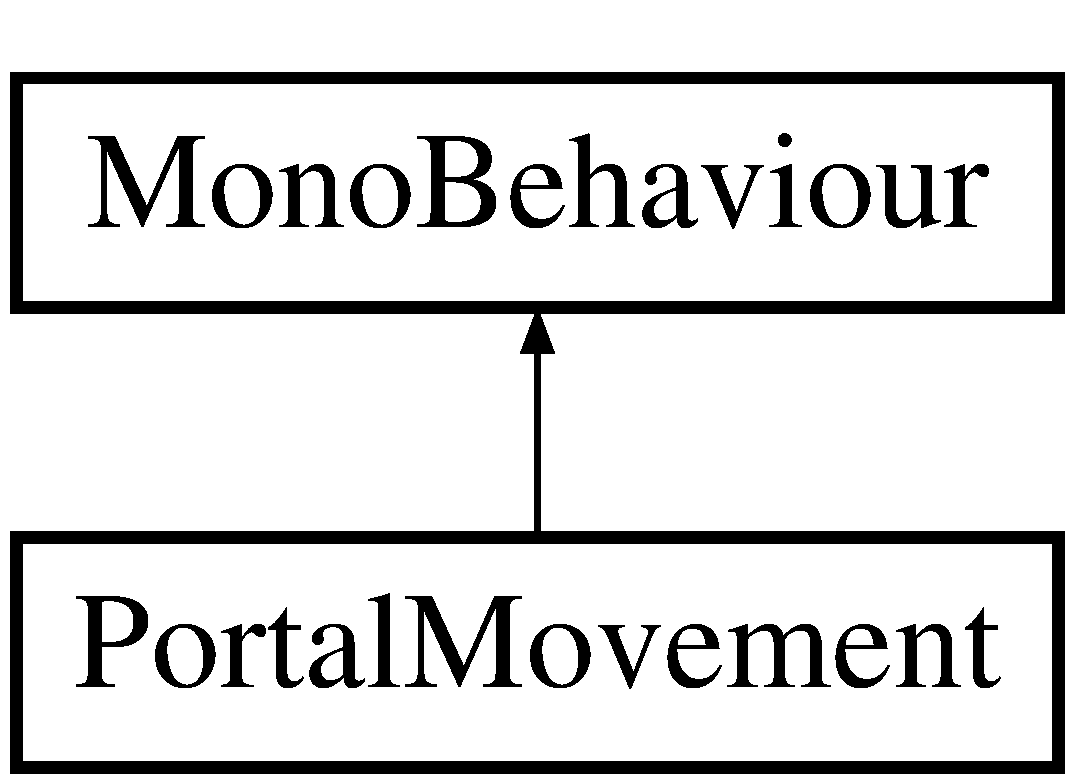
\includegraphics[height=2.000000cm]{class_portal_movement}
\end{center}
\end{figure}
\subsection*{Public Member Functions}
\begin{DoxyCompactItemize}
\item 
void \mbox{\hyperlink{class_portal_movement_aa7beca3afea663ec0de74142ac852ca4}{Start}} ()
\item 
\mbox{\Hypertarget{class_portal_movement_aeb23b9ab7c546f248da82c6e9b6dd473}\label{class_portal_movement_aeb23b9ab7c546f248da82c6e9b6dd473}} 
void {\bfseries Update} ()
\item 
void \mbox{\hyperlink{class_portal_movement_aa7beca3afea663ec0de74142ac852ca4}{Start}} ()
\item 
\mbox{\Hypertarget{class_portal_movement_aeb23b9ab7c546f248da82c6e9b6dd473}\label{class_portal_movement_aeb23b9ab7c546f248da82c6e9b6dd473}} 
void {\bfseries Update} ()
\end{DoxyCompactItemize}
\subsection*{Public Attributes}
\begin{DoxyCompactItemize}
\item 
\mbox{\Hypertarget{class_portal_movement_ad02d06d822cb837c2b6815bd0f448ca7}\label{class_portal_movement_ad02d06d822cb837c2b6815bd0f448ca7}} 
Vector2 {\bfseries target}
\item 
\mbox{\Hypertarget{class_portal_movement_a527ecae1396a95f37468482a7e717211}\label{class_portal_movement_a527ecae1396a95f37468482a7e717211}} 
Rigidbody2D {\bfseries rb}
\item 
\mbox{\Hypertarget{class_portal_movement_a206e9a3b0b782c6fd112bf99ff6a7bf4}\label{class_portal_movement_a206e9a3b0b782c6fd112bf99ff6a7bf4}} 
float {\bfseries speed} = 30f
\item 
\mbox{\Hypertarget{class_portal_movement_a80572fcf6a3158f6cc7fe64ed4d68f20}\label{class_portal_movement_a80572fcf6a3158f6cc7fe64ed4d68f20}} 
Vector2 {\bfseries move\+Direction}
\end{DoxyCompactItemize}


\subsection{Detailed Description}
Handles portal bullet movement. 

\subsection{Member Function Documentation}
\mbox{\Hypertarget{class_portal_movement_aa7beca3afea663ec0de74142ac852ca4}\label{class_portal_movement_aa7beca3afea663ec0de74142ac852ca4}} 
\index{Portal\+Movement@{Portal\+Movement}!Start@{Start}}
\index{Start@{Start}!Portal\+Movement@{Portal\+Movement}}
\subsubsection{\texorpdfstring{Start()}{Start()}\hspace{0.1cm}{\footnotesize\ttfamily [1/2]}}
{\footnotesize\ttfamily void Portal\+Movement.\+Start (\begin{DoxyParamCaption}{ }\end{DoxyParamCaption})\hspace{0.3cm}{\ttfamily [inline]}}

Method is in charge of the portal bullet movement. \begin{DoxyPrecond}{Precondition}
portal is shot 
\end{DoxyPrecond}
\begin{DoxyPostcond}{Postcondition}
portal bullet moves to the location of the mouse when it was clicked until it collides with a valid object 
\end{DoxyPostcond}
\mbox{\Hypertarget{class_portal_movement_aa7beca3afea663ec0de74142ac852ca4}\label{class_portal_movement_aa7beca3afea663ec0de74142ac852ca4}} 
\index{Portal\+Movement@{Portal\+Movement}!Start@{Start}}
\index{Start@{Start}!Portal\+Movement@{Portal\+Movement}}
\subsubsection{\texorpdfstring{Start()}{Start()}\hspace{0.1cm}{\footnotesize\ttfamily [2/2]}}
{\footnotesize\ttfamily void Portal\+Movement.\+Start (\begin{DoxyParamCaption}{ }\end{DoxyParamCaption})\hspace{0.3cm}{\ttfamily [inline]}}

Method is in charge of the portal bullet movement. \begin{DoxyPrecond}{Precondition}
portal is shot 
\end{DoxyPrecond}
\begin{DoxyPostcond}{Postcondition}
portal bullet moves to the location of the mouse when it was clicked until it collides with a valid object 
\end{DoxyPostcond}


The documentation for this class was generated from the following file\+:\begin{DoxyCompactItemize}
\item 
Assets/\+Scripts/Portal\+Movement.\+cs\end{DoxyCompactItemize}

\hypertarget{class_shoot_portal}{}\section{Shoot\+Portal Class Reference}
\label{class_shoot_portal}\index{Shoot\+Portal@{Shoot\+Portal}}
Inheritance diagram for Shoot\+Portal\+:\begin{figure}[H]
\begin{center}
\leavevmode
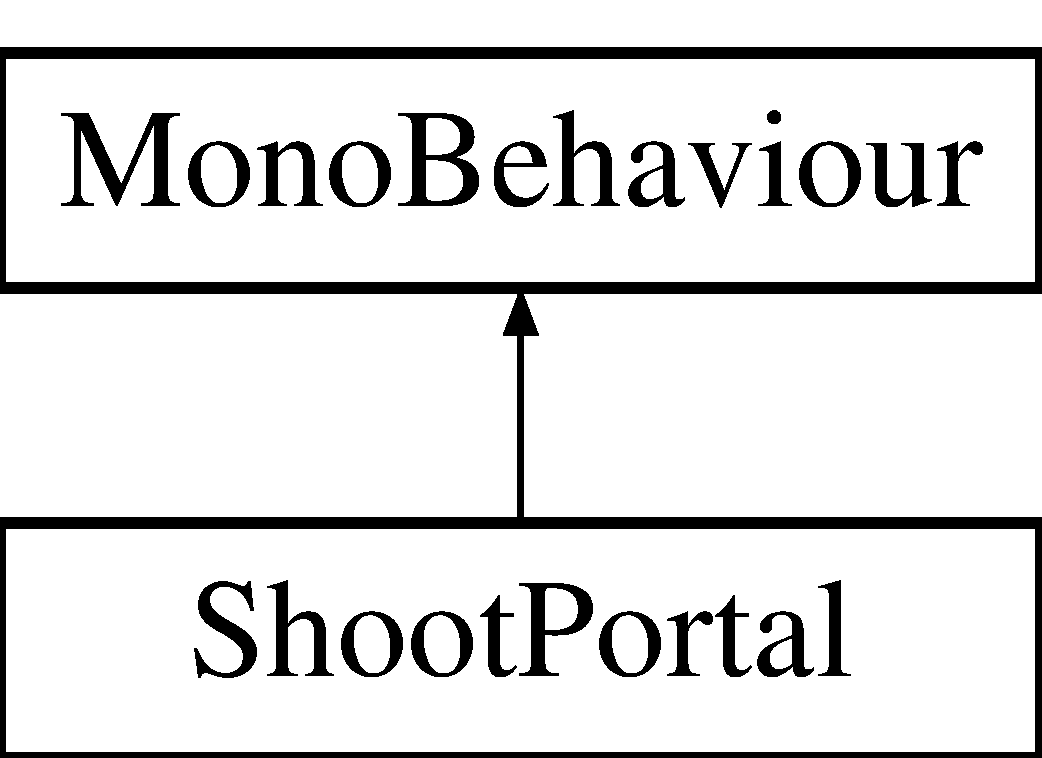
\includegraphics[height=2.000000cm]{class_shoot_portal}
\end{center}
\end{figure}
\subsection*{Public Member Functions}
\begin{DoxyCompactItemize}
\item 
\mbox{\Hypertarget{class_shoot_portal_afb543600d8358d399c285b327093a922}\label{class_shoot_portal_afb543600d8358d399c285b327093a922}} 
void {\bfseries Start} ()
\item 
void \mbox{\hyperlink{class_shoot_portal_a1160266ce719d6b93655286e0909bae8}{Update}} ()
\end{DoxyCompactItemize}
\subsection*{Public Attributes}
\begin{DoxyCompactItemize}
\item 
\mbox{\Hypertarget{class_shoot_portal_a715a70a24a5337424fc183a04cc0a3d2}\label{class_shoot_portal_a715a70a24a5337424fc183a04cc0a3d2}} 
Game\+Object {\bfseries blue\+Portal}
\item 
\mbox{\Hypertarget{class_shoot_portal_ad355d40bf4cc38c8deeb65c71c8b1d13}\label{class_shoot_portal_ad355d40bf4cc38c8deeb65c71c8b1d13}} 
Game\+Object {\bfseries red\+Portal}
\item 
\mbox{\Hypertarget{class_shoot_portal_ab1052b79920f7bdb495e3cc8af5d429d}\label{class_shoot_portal_ab1052b79920f7bdb495e3cc8af5d429d}} 
Vector2 {\bfseries velocity}
\end{DoxyCompactItemize}


\subsection{Detailed Description}
Handles portal shooting. 

\subsection{Member Function Documentation}
\mbox{\Hypertarget{class_shoot_portal_a1160266ce719d6b93655286e0909bae8}\label{class_shoot_portal_a1160266ce719d6b93655286e0909bae8}} 
\index{Shoot\+Portal@{Shoot\+Portal}!Update@{Update}}
\index{Update@{Update}!Shoot\+Portal@{Shoot\+Portal}}
\subsubsection{\texorpdfstring{Update()}{Update()}}
{\footnotesize\ttfamily void Shoot\+Portal.\+Update (\begin{DoxyParamCaption}{ }\end{DoxyParamCaption})\hspace{0.3cm}{\ttfamily [inline]}}

shoots a portal when mouse is clicked following the direction towards the location of the mouse pointer when clicked. \begin{DoxyPrecond}{Precondition}
mouse is clicked 
\end{DoxyPrecond}
\begin{DoxyPostcond}{Postcondition}
portal is shot 
\end{DoxyPostcond}


The documentation for this class was generated from the following file\+:\begin{DoxyCompactItemize}
\item 
Assets/\+Scripts/Shoot\+Portal.\+cs\end{DoxyCompactItemize}

\hypertarget{class_teleport_player}{}\section{Teleport\+Player Class Reference}
\label{class_teleport_player}\index{Teleport\+Player@{Teleport\+Player}}
Inheritance diagram for Teleport\+Player\+:\begin{figure}[H]
\begin{center}
\leavevmode
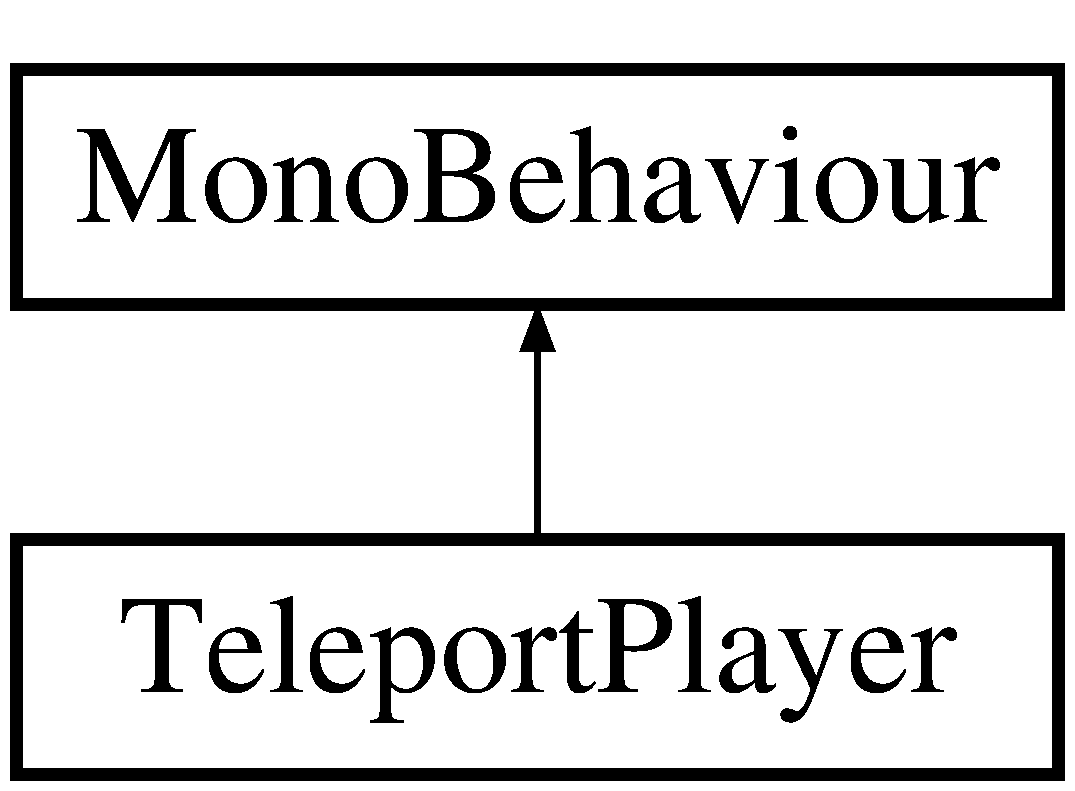
\includegraphics[height=2.000000cm]{class_teleport_player}
\end{center}
\end{figure}
\subsection*{Public Member Functions}
\begin{DoxyCompactItemize}
\item 
void \mbox{\hyperlink{class_teleport_player_a555b0c226c512d6bc9ce347b19957cd9}{On\+Trigger\+Enter2D}} (Collider2D collision)
\item 
void \mbox{\hyperlink{class_teleport_player_addd6af261867cf134ac87c580cebec92}{On\+Trigger\+Exit2D}} (Collider2D collision)
\item 
\mbox{\Hypertarget{class_teleport_player_ad75d1699964434878bf8a31244a6a4af}\label{class_teleport_player_ad75d1699964434878bf8a31244a6a4af}} 
void {\bfseries Start} ()
\item 
\mbox{\Hypertarget{class_teleport_player_ab8dc957d5f4ca8e3bee2d4b48ac0ed23}\label{class_teleport_player_ab8dc957d5f4ca8e3bee2d4b48ac0ed23}} 
void {\bfseries Update} ()
\item 
void \mbox{\hyperlink{class_teleport_player_a1ab94b6c3d13f1287f9127393afe2298}{On\+Collision\+Enter2D}} (Collision2D collision)
\item 
void \mbox{\hyperlink{class_teleport_player_ac85fc2322d2dc27de518434422c2c25e}{On\+Collision\+Exit2D}} (Collision2D collision)
\end{DoxyCompactItemize}
\subsection*{Public Attributes}
\begin{DoxyCompactItemize}
\item 
\mbox{\Hypertarget{class_teleport_player_a3a1f027838b709b22b058dd5d8a4a140}\label{class_teleport_player_a3a1f027838b709b22b058dd5d8a4a140}} 
string {\bfseries portal\+Entered}
\end{DoxyCompactItemize}


\subsection{Detailed Description}
Handles player teleporting

Handles teleporting players between portals. 

\subsection{Member Function Documentation}
\mbox{\Hypertarget{class_teleport_player_a1ab94b6c3d13f1287f9127393afe2298}\label{class_teleport_player_a1ab94b6c3d13f1287f9127393afe2298}} 
\index{Teleport\+Player@{Teleport\+Player}!On\+Collision\+Enter2D@{On\+Collision\+Enter2D}}
\index{On\+Collision\+Enter2D@{On\+Collision\+Enter2D}!Teleport\+Player@{Teleport\+Player}}
\subsubsection{\texorpdfstring{On\+Collision\+Enter2\+D()}{OnCollisionEnter2D()}}
{\footnotesize\ttfamily void Teleport\+Player.\+On\+Collision\+Enter2D (\begin{DoxyParamCaption}\item[{Collision2D}]{collision }\end{DoxyParamCaption})\hspace{0.3cm}{\ttfamily [inline]}}

This method runs after registering collision of player with portal and its goal is to switch the position of the player to that one of the other portal. pre\+: portals are created within an appropiate surface post\+: after player enters a portal it\textquotesingle{}s position changes to that of the other portal \mbox{\Hypertarget{class_teleport_player_ac85fc2322d2dc27de518434422c2c25e}\label{class_teleport_player_ac85fc2322d2dc27de518434422c2c25e}} 
\index{Teleport\+Player@{Teleport\+Player}!On\+Collision\+Exit2D@{On\+Collision\+Exit2D}}
\index{On\+Collision\+Exit2D@{On\+Collision\+Exit2D}!Teleport\+Player@{Teleport\+Player}}
\subsubsection{\texorpdfstring{On\+Collision\+Exit2\+D()}{OnCollisionExit2D()}}
{\footnotesize\ttfamily void Teleport\+Player.\+On\+Collision\+Exit2D (\begin{DoxyParamCaption}\item[{Collision2D}]{collision }\end{DoxyParamCaption})\hspace{0.3cm}{\ttfamily [inline]}}

Resets the state of the player after its position is changed between the portals. \mbox{\Hypertarget{class_teleport_player_a555b0c226c512d6bc9ce347b19957cd9}\label{class_teleport_player_a555b0c226c512d6bc9ce347b19957cd9}} 
\index{Teleport\+Player@{Teleport\+Player}!On\+Trigger\+Enter2D@{On\+Trigger\+Enter2D}}
\index{On\+Trigger\+Enter2D@{On\+Trigger\+Enter2D}!Teleport\+Player@{Teleport\+Player}}
\subsubsection{\texorpdfstring{On\+Trigger\+Enter2\+D()}{OnTriggerEnter2D()}}
{\footnotesize\ttfamily void Teleport\+Player.\+On\+Trigger\+Enter2D (\begin{DoxyParamCaption}\item[{Collider2D}]{collision }\end{DoxyParamCaption})\hspace{0.3cm}{\ttfamily [inline]}}

This method runs after registering collision of player with portal and its goal is to switch the position of the player to that one of the other portal \begin{DoxyPrecond}{Precondition}
portals are created within an appropiate surface 
\end{DoxyPrecond}
\begin{DoxyPostcond}{Postcondition}
after player enters a portal it\textquotesingle{}s position changes to that of the other portal 
\end{DoxyPostcond}

\begin{DoxyParams}{Parameters}
{\em collision} & collision object created by the physics engine \\
\hline
\end{DoxyParams}
\mbox{\Hypertarget{class_teleport_player_addd6af261867cf134ac87c580cebec92}\label{class_teleport_player_addd6af261867cf134ac87c580cebec92}} 
\index{Teleport\+Player@{Teleport\+Player}!On\+Trigger\+Exit2D@{On\+Trigger\+Exit2D}}
\index{On\+Trigger\+Exit2D@{On\+Trigger\+Exit2D}!Teleport\+Player@{Teleport\+Player}}
\subsubsection{\texorpdfstring{On\+Trigger\+Exit2\+D()}{OnTriggerExit2D()}}
{\footnotesize\ttfamily void Teleport\+Player.\+On\+Trigger\+Exit2D (\begin{DoxyParamCaption}\item[{Collider2D}]{collision }\end{DoxyParamCaption})\hspace{0.3cm}{\ttfamily [inline]}}

Resets the state of the player after its position is changed between the portals 
\begin{DoxyParams}{Parameters}
{\em collision} & collision object created by the physics engine \\
\hline
\end{DoxyParams}


The documentation for this class was generated from the following file\+:\begin{DoxyCompactItemize}
\item 
Assets/\+Scripts/Teleport\+Player.\+cs\end{DoxyCompactItemize}

\hypertarget{class_win_game}{}\section{Win\+Game Class Reference}
\label{class_win_game}\index{Win\+Game@{Win\+Game}}
Inheritance diagram for Win\+Game\+:\begin{figure}[H]
\begin{center}
\leavevmode
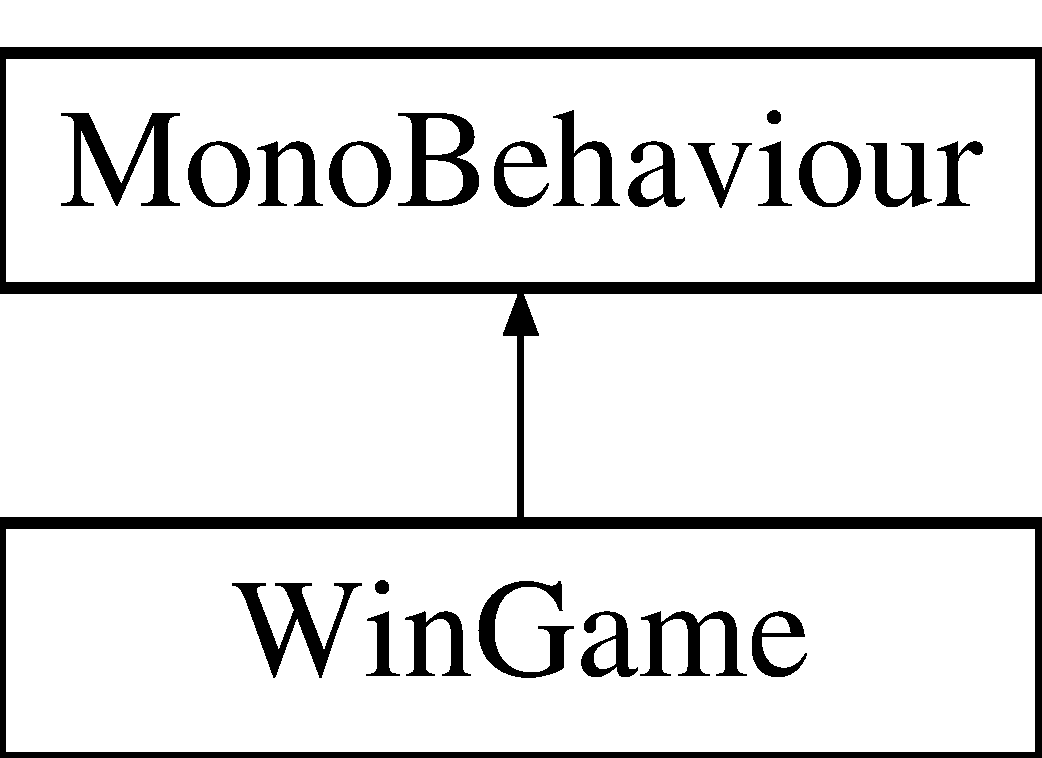
\includegraphics[height=2.000000cm]{class_win_game}
\end{center}
\end{figure}
\subsection*{Public Member Functions}
\begin{DoxyCompactItemize}
\item 
void \mbox{\hyperlink{class_win_game_a20f3871fd050c6da54d041b49a7fb063}{On\+Collision\+Enter2D}} (Collision2D collision)
\item 
void \mbox{\hyperlink{class_win_game_a20f3871fd050c6da54d041b49a7fb063}{On\+Collision\+Enter2D}} (Collision2D collision)
\end{DoxyCompactItemize}
\subsection*{Public Attributes}
\begin{DoxyCompactItemize}
\item 
\mbox{\Hypertarget{class_win_game_a786a1f699b803e4eafe16804002e4f18}\label{class_win_game_a786a1f699b803e4eafe16804002e4f18}} 
Game\+Object {\bfseries you\+Win}
\end{DoxyCompactItemize}


\subsection{Detailed Description}
Handles completion of level. 

\subsection{Member Function Documentation}
\mbox{\Hypertarget{class_win_game_a20f3871fd050c6da54d041b49a7fb063}\label{class_win_game_a20f3871fd050c6da54d041b49a7fb063}} 
\index{Win\+Game@{Win\+Game}!On\+Collision\+Enter2D@{On\+Collision\+Enter2D}}
\index{On\+Collision\+Enter2D@{On\+Collision\+Enter2D}!Win\+Game@{Win\+Game}}
\subsubsection{\texorpdfstring{On\+Collision\+Enter2\+D()}{OnCollisionEnter2D()}\hspace{0.1cm}{\footnotesize\ttfamily [1/2]}}
{\footnotesize\ttfamily void Win\+Game.\+On\+Collision\+Enter2D (\begin{DoxyParamCaption}\item[{Collision2D}]{collision }\end{DoxyParamCaption})\hspace{0.3cm}{\ttfamily [inline]}}

Sets win state to true. \begin{DoxyPrecond}{Precondition}
Player reaches the door object 
\end{DoxyPrecond}
\begin{DoxyPostcond}{Postcondition}
Success message is displayed indicating level completed After Player \char`\"{}collides\char`\"{} with door object it will display a Win message indicating level completion 
\end{DoxyPostcond}
\mbox{\Hypertarget{class_win_game_a20f3871fd050c6da54d041b49a7fb063}\label{class_win_game_a20f3871fd050c6da54d041b49a7fb063}} 
\index{Win\+Game@{Win\+Game}!On\+Collision\+Enter2D@{On\+Collision\+Enter2D}}
\index{On\+Collision\+Enter2D@{On\+Collision\+Enter2D}!Win\+Game@{Win\+Game}}
\subsubsection{\texorpdfstring{On\+Collision\+Enter2\+D()}{OnCollisionEnter2D()}\hspace{0.1cm}{\footnotesize\ttfamily [2/2]}}
{\footnotesize\ttfamily void Win\+Game.\+On\+Collision\+Enter2D (\begin{DoxyParamCaption}\item[{Collision2D}]{collision }\end{DoxyParamCaption})\hspace{0.3cm}{\ttfamily [inline]}}

Sets win state to true. \begin{DoxyPrecond}{Precondition}
Player reaches the door object 
\end{DoxyPrecond}
\begin{DoxyPostcond}{Postcondition}
Success message is displayed indicating level completed After Player \char`\"{}collides\char`\"{} with door object it will display a Win message indicating level completion 
\end{DoxyPostcond}

\begin{DoxyParams}{Parameters}
{\em collision} & collision object created by the physics engine \\
\hline
\end{DoxyParams}


The documentation for this class was generated from the following file\+:\begin{DoxyCompactItemize}
\item 
Assets/\+Scripts/Win\+Game.\+cs\end{DoxyCompactItemize}

%--- End generated contents ---

% Index
\backmatter
\newpage
\phantomsection
\clearemptydoublepage
\addcontentsline{toc}{chapter}{Index}
\printindex

\end{document}
